%\subsection*{Introduction}
\showCILC{true}{
	\begin{frame}{Introduction}
	\onslide<1->{
		\begin{block}{Epistemic Reasoning}
			Reasoning not only about agents' \emphSlide{perception of the world} but also about agents' \emphSlide{knowledge} and/or \emphSlide{beliefs} of her and others' beliefs.
		\end{block}
	}

	\onslide<2->{
		\begin{block}{Multi-agent Epistemic Planning Problem~\cite{bolander2011epistemic}}
			Finding \emphSlide{plans} where the goals can refer to:
			\begin{itemize}
				\item [-] the state of the world
				\item [-] the knowledge and/or the  beliefs  of the agents
			\end{itemize}
		\end{block}
	}

	\end{frame}
}

\showCILC{true}{
	\begin{frame}{An Example}
		\onslide<2->{
			\begin{exampleblock}{Initial State}
				\begin{itemize}
					\item[-] 	\agentSlide{Snoopy} and \agentSlide{Charlie} are \ttSlide{looking} while  \agentSlide{Lucy} is \ttSlide{$\neg$looking}
					\item[-] 	No one knows the \ttSlide{coin position}.
				\end{itemize}
			\end{exampleblock}
		}
		\onslide<1->{
			\centering
			
\includegraphics[width=0.8\textwidth]{img/initial_state}
		}
	\end{frame}
}

\showCILC{true}{
	\begin{frame}{An Example}

		\begin{exampleblock}{Goal State}
			\begin{itemize}
				\item[-] \agentSlide{Charlie} knows the \ttSlide{coin position}\\
				\item[-] \agentSlide{Lucy} knows that \agentSlide{Charlie} knows the \ttSlide{coin position}\\
				\item[-] \agentSlide{Snoopy} does not know anything about the plan execution\\
			\end{itemize}
		\end{exampleblock}
		\centering
		
\includegraphics[width=0.8\textwidth]{img/goal_state}
	\end{frame}
}


\showCILC{true}{
	\begin{frame}{Challenges}
		\begin{columns}
			\begin{column}{0.8\textwidth}
				\begin{center}
					An \agentSlide{agent} has to reason about his actions effects on
					\begin{itemize}
						\item[-] The \emphSlide{state of the world}\\
						\item[-] The \agentSlide{agents}' awareness of the environment\\
						\item[-] The \agentSlide{agents}' awareness of other \agentSlide{agents}' \emphSlide{actions}\\
						\item[-] The knowledge of other \agentSlide{agents} about his own\\
					\end{itemize}
				\end{center}
			\end{column}

			\begin{column}{0.3\textwidth}
				\centering
				\includegraphics[width=0.8\textwidth]{img/confused_charlie}
			\end{column}
		\end{columns}
	\end{frame}
}


%\subsection*{Problem Formalization}
\showCILC{true}{
	\begin{frame}{Notations}
		Given a set of \agentSlide{agents} \sAG\
		%	\onslide<1->{
		%		\begin{tikzpicture}[remember picture,overlay]
		%		\node[xshift=-5.1cm,yshift=-4cm] (A) at (current page.north east){};
		%		\node[xshift=-1.0cm,yshift=-3.5cm] (B) at (current page.north east){\NWFSGreen{Belief}};
		%		\draw[] (B)-- +(0,-0.7);
		%		\draw[to path={-| (\tikztotarget)}] (B)+(0,-0.7) edge  (A);
		%		\end{tikzpicture}%}
		\onslide<1->{

			\begin{block}{Modal operator $\bBSlide{ag}{}$ \hfill {\footnotesize where \texttt{ag} $\in$ \sAG}}
				Models the beliefs of \agentSlide{ag} about the \ttSlide{state of the world} and/or about the beliefs of other \agentSlide{agents}.
			\end{block}}
		\onslide<2->{
			\begin{block}{Group operator $\cAlpha{}$ \hfill {\footnotesize where $\alpha \subseteq$ \sAG}}
				Expresses the \emphSlide{common belief} of a group of \agentSlide{agents}.
			\end{block}}
		\onslide<3->{
			\begin{block}{Belief Formulae}
				Take into consideration \emphSlide{fluents} and/or \agentSlide{agents}' beliefs.
			\end{block}}
	\end{frame}
}

\showCILC{true}{
	\begin{frame}{Example of Belief Formulae}

		\begin{columns}
			\hspace*{0.8cm}\begin{column}{0.8\textwidth}
				Given
				\begin{itemize}
					\item[-] \sAG\ $= \{\agentSlide{Snoopy},\agentSlide{Charlie},\agentSlide{Lucy}\}$
					\item[-] \sF~~~$= \{\ttSlide{opened},\ttSlide{head},\ttSlide{looking}_{\agentSlide{ag}}\}~\agentSlide{ag} \in \sAG$
				\end{itemize}
			\end{column}
			\begin{column}{0.3\textwidth}
				\hspace*{-0.6cm}
				
\includegraphics[width=1.0\textwidth]{img/initial_state}
			\end{column}
		\end{columns}
		~\newline
		\begin{exampleblock}{$\bBSlide{Snoopy}{\bBSlide{Charlie}{\neg \text{\texttt{opened}}}}$}
			\agentSlide{Snoopy} believes that \agentSlide{Charlie} believes that the box is \ttSlide{$\neg$opened}.
		\end{exampleblock}

		\onslide<2>{\begin{exampleblock}{$\cAlpha{(\neg\bBSlide{Lucy}{\mathtt{heads}} \wedge \neg \bBSlide{Lucy}{\neg \mathtt{head}})}$ \hfill {\footnotesize where $\alpha=\sAG$}}
				It is \ck\ that \agentSlide{Lucy} does not know whether the coin lies \ttSlide{heads} or \ttSlide{tails} up
			\end{exampleblock}}
	\end{frame}
}

\subsection*{}
\showCILC{true}{
	\begin{frame}{Knowledge vs. Belief}
		\begin{itemize}
			\item[-] The modal operator $\bBSlide{\agentSlide{ag}}{}$ represents the worlds' relation
			\item[-] Different relation's properties imply different meaning for $\bBSlide{\agentSlide{ag}}{}$
			      \only<2>{\item[-] \emphSlide{$\mathcal{K}$nowledge} and \emphSlide{$\mathcal{B}$elief} are characterized by a subset of the following axioms}
		\end{itemize}
		\vfill
		\only<+>{
			\begin{figure}
				\begin{subfigure}{0.5\textwidth}
					\centering
					%	\hspace*{-0.5cm}
					
\includegraphics[width=0.6\textwidth]{img/sunny2}
				\end{subfigure}%
				\begin{subfigure}{0.5\textwidth}
					\centering
					%\vspace*{0.7cm}
					%\hspace*{-0.6cm}
					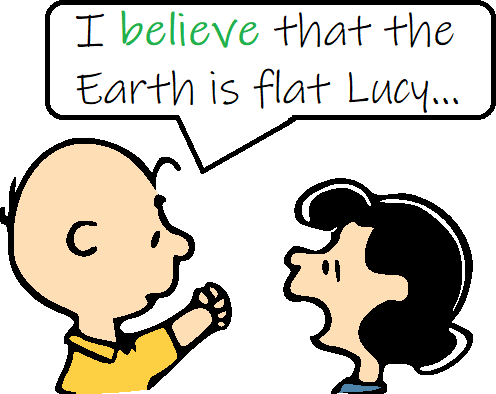
\includegraphics[width=0.8\textwidth]{img/flatearth}
				\end{subfigure}
			\end{figure}

		}
		\only<+>{\begin{block}{Serial (\textbf{D}) and S5 (\textbf{K,T,4,5}) Axioms}
				Given the fluent formulae $\phi$, $\psi$ and the worlds \texttt{i}, \texttt{j}
				\begin{itemize}
					\item[D] $\neg \calR_{\mathtt{i}} \bot$ \hfill  {\emphSlide{$\mathcal{B~K}$}}
					\item[K] $(\calR_{\mathtt{i}}\varphi \wedge \calR_{\mathtt{i}}(\varphi \implies \psi)) \implies  \calR_{\mathtt{i}}\psi$ \hfill {\emphSlide{$\mathcal{B~K}$}}
					\item[T] $\calR_{\mathtt{i}}\varphi  \implies \varphi$ \hfill {\emphSlide{$\mathcal{K}$}}
					\item[4] $\calR_{\mathtt{i}}\varphi  \implies \calR_{\mathtt{i}}\calR_{\mathtt{i}}\varphi$ \hfill {\emphSlide{$\mathcal{B~K}$}}
					\item[5] $\neg \calR_{\mathtt{i}}\varphi  \implies \calR_{\mathtt{i}}\neg \calR_{\mathtt{i}}\varphi$ \hfill {\emphSlide{$\mathcal{B~K}$}}
				\end{itemize}
			\end{block}}
	\end{frame}
}
